\documentclass[11pt,a4paper]{article}

% ============================================================
% PACKAGES
% ============================================================
\usepackage[utf8]{inputenc}
\usepackage[T1]{fontenc}
\usepackage{lmodern}
\usepackage[margin=1in]{geometry}
\usepackage{amsmath,amssymb,amsthm}
\usepackage{graphicx}
\usepackage{xcolor}
\usepackage{hyperref}
\usepackage{cleveref}
\usepackage{booktabs}
\usepackage{multirow}
\usepackage{tikz}
\usepackage{pgfplots}
\usepackage{listings}
\usepackage{caption}
\usepackage{subcaption}
\usepackage{enumitem}
\usepackage{float}
\usepackage{url}

\emergencystretch=3em

\pgfplotsset{compat=1.18}
\usetikzlibrary{arrows.meta, positioning, calc, fit, backgrounds, shapes.geometric}

\hypersetup{
    colorlinks=true,
    linkcolor=blue!70!black,
    citecolor=green!50!black,
    urlcolor=blue!60!black
}

% ============================================================
% LISTING STYLE (Rust)
% ============================================================
\lstdefinelanguage{Rust}{
  keywords={fn, let, mut, pub, struct, impl, trait, use, mod, self, Self,
            if, else, for, while, loop, match, return, where, in, as,
            true, false, Some, None, Ok, Err, Vec, usize, f32, u8, bool},
  morecomment=[l]{//},
  morecomment=[s]{/*}{*/},
  morestring=[b]",
  sensitive=true,
}
\lstset{
  language=Rust,
  basicstyle=\ttfamily\footnotesize,
  keywordstyle=\color{blue!70!black}\bfseries,
  commentstyle=\color{green!50!black}\itshape,
  stringstyle=\color{red!60!black},
  numbers=left,
  numberstyle=\tiny\color{gray},
  breaklines=true,
  frame=single,
  rulecolor=\color{gray!30},
  backgroundcolor=\color{gray!5},
  captionpos=b,
}

% ============================================================
% THEOREM ENVIRONMENTS
% ============================================================
\newtheorem{theorem}{Theorem}[section]
\newtheorem{definition}[theorem]{Definition}
\newtheorem{proposition}[theorem]{Proposition}
\theoremstyle{remark}
\newtheorem{remark}{Remark}[section]

% ============================================================
% TITLE
% ============================================================
\title{\textbf{Observer-Independent 3D Simulation and Topological Preservation Across Projection Boundaries}}

\author{
  Ryan J. Cardwell \\
  Crystalline Labs LLC, Milton, FL, USA \\
  ORCID: \href{https://orcid.org/0009-0005-0307-0746}{0009-0005-0307-0746}
}

\date{March 2026}

% ============================================================
% DOCUMENT
% ============================================================
\begin{document}
\maketitle

% ============================================================
% ABSTRACT
% ============================================================
\begin{abstract}
Current 3D game engines store geometry in three-dimensional data structures but compute on lower-dimensional manifolds at nearly every pipeline stage: navigation meshes are 2D simplicial complexes, collision detection operates on 2D surfaces with 1D winding-number inference, broadphase uses axis-aligned bounding boxes with trivial topology, and rendering projects to a 2D framebuffer through observer-dependent culling. This paper presents a minimal engine architecture that enforces a hard separation between an observer-independent simulation (``System~1'') and an observation apparatus (``System~2'') that exists as an object inside the simulation and queries it through a formally defined API boundary. We implement this architecture in Rust, construct a solid torus in a sparse voxel grid with forward photon-mapped illumination, verify that the boundary operator on the cubical complex satisfies $\partial^2 = 0$, confirm that the solid torus has Betti number $\beta_1 = 1$ (the hole exists), and then measure whether this topological feature survives projection through the observation boundary into System~2's depth map. We find a phase transition: at observer distances $\leq 15$\,m, the hole is recovered at all tested image resolutions ($32^2$ through $512^2$); at 20\,m, the hole vanishes at all resolutions. The critical threshold is parameterized by a dimensionless geometric ratio $\Gamma = (R - r)/d \approx 0.08$--$0.10$, is distance-dependent and resolution-independent, ruling out sampling-rate explanations. All results are reproducible from the companion codebase in under five minutes on commodity hardware.
\end{abstract}

\vspace{1em}
\noindent\textbf{Keywords:} computational topology, observer-independent simulation, cubical homology, Betti numbers, game engine architecture, topological phase transition

% ============================================================
% 5Ws + H
% ============================================================
\section{Direct, Indirect, and Higher-Order 5Ws + H}
\label{sec:5wh}

\subsection*{What}

Every 3D video game you have ever played has lied to you. Not about the story or the graphics---about the \emph{three} in 3D. The game stores objects with three-dimensional coordinates, yes. But when it actually computes---when it figures out whether you can walk somewhere, whether a bullet hits a wall, whether light bounces off a surface---it drops to two dimensions or less. The navigation mesh your character walks on is a flat sheet draped over the terrain, like a tablecloth over a table. The physics engine checks collisions by wrapping objects in boxes aligned to the X, Y, and Z axes independently---three separate one-dimensional checks, not a three-dimensional one. And the image you see on screen is the result of a massive dimensional collapse: the entire 3D world, projected through a virtual camera, crushed into a grid of colored pixels on a flat monitor.

None of this is a secret. Every game developer knows it. The question nobody has formally asked is: \emph{what gets destroyed in the collapse?}

This paper answers that question using topology---the branch of mathematics that studies properties of shapes that survive continuous deformation. Specifically, we study \emph{holes}. A torus (the shape of a donut) has a hole through its center. That hole is a topological feature: you can stretch the torus, squeeze it, twist it, but the hole persists as long as you don't tear or glue. In mathematical language, the torus has a non-trivial first homology group, written $H_1 \neq 0$. The hole is detected by finding a loop on the torus that cannot be shrunk to a point---a loop that threads through the hole.

We built a minimal 3D engine with a hard rule: the simulation runs without knowing whether anyone is looking at it. There is no camera inside the simulation. No frustum culling. No level-of-detail reduction. The torus exists whether you observe it or not. Then we built a separate observation system---a virtual camera that exists as an object \emph{inside} the simulation and queries it the way a retina samples photons: by casting rays and measuring what comes back.

The question: does the hole survive the observation? Does the topological feature that exists in the simulation persist after being projected through the camera into a flat depth image?

The answer: sometimes. There is a critical distance. Closer than about 15 meters, the hole is detectable from the depth map at every image resolution we tested, even $32\times32$ pixels. Farther than 20 meters, the hole vanishes from the depth map at every resolution, even $512\times512$. The transition is sharp. And critically, it is \emph{not} a resolution effect---making the image bigger does not help. What matters is the geometric relationship between the observer and the hole. Stand close enough and you see it. Stand too far and it disappears, no matter how good your eyes are.

\subsection*{Why}

Because the thing that determines whether you can perceive a topological feature is not the quality of your instrument. It is your position relative to the feature. This has implications that extend well beyond video games.

In computer graphics, it means that the standard approach of improving visual fidelity through higher resolution, more polygons, better shaders, and ray tracing does not address the fundamental topological limitations of observer-dependent rendering.

In computational physics, it means that simulations which optimize by skipping computation where ``nobody is looking'' may be introducing topological errors that propagate silently. A rope simulation that uses 2D surface contacts cannot detect whether a knot is a trefoil or an unknot.

In the study of observation itself, this result provides a concrete, measurable, reproducible demonstration of a phenomenon that philosophy and cognitive science have long discussed abstractly: the act of observation does not passively record reality. It \emph{projects} reality through an apparatus, and the projection has a topology that may differ from the source. What you see depends on where you stand. This is not a metaphor. It is a theorem with a proof and a codebase.

\subsection*{Who}

This work was produced by a single researcher using a human-AI collaborative methodology. The entire codebase---approximately 1,200 lines of Rust---was written in a single session of roughly ten hours. The human operator (the author) provided the architectural design, the research questions, the connection to algebraic topology, and the experimental design. The AI collaborator (Claude, Anthropic) provided the implementation, debugging, and computational execution.

\subsection*{When}

Now. The code compiles today. The results reproduce today. The companion repository is archived on Zenodo with a DOI. Nothing in this paper requires future hardware, future algorithms, or future theoretical developments.

\subsection*{Where}

The computation happens in two places that never touch. System~1 builds a sparse voxel grid, evaluates a signed distance field, propagates photons forward, and computes homology. System~2 generates rays from a pinhole camera model, queries System~1 through a trait interface, and assembles depth maps. The API boundary is enforced at compile time by Rust's module visibility system. The observer cannot contaminate the simulation because the compiler will not allow it.

\subsection*{How}

By treating the boundary operator $\partial$ as the fundamental diagnostic tool. The composition $\partial_{k-1} \circ \partial_k = 0$---``the boundary of a boundary is zero''---is verified explicitly at both composition levels of the cubical complex. If $\partial^2 \neq 0$ in the implementation, there is a bug, not a finding.

\subsection*{Higher-Order}

The standard model of rendering treats the observer as a privileged entity. The entire computational pipeline is organized around what the camera can see. This paper demonstrates an alternative: the world exists first, the observer samples it second, and the sampling process has measurable topological consequences. The finding that the critical threshold is distance-dependent rather than resolution-dependent suggests something about the nature of topological perception itself. A hole is a global feature. Whether that global feature is detectable through a local observation depends on geometry, not fidelity.

% ============================================================
% INTRODUCTION
% ============================================================
\section{Introduction}
\label{sec:intro}

\subsection{The Problem}

Modern 3D game engines are architecturally organized around the observer. The rendering pipeline begins with the camera: the view frustum defines which objects are visible, level-of-detail (LOD) systems select geometric complexity based on screen-space projected size, and occlusion culling eliminates objects hidden behind others. Even physics simulation is observer-coupled: many engines implement ``physics sleep'' for objects far from active gameplay regions, and Unreal Engine~5's Nanite system explicitly makes rendering cost proportional to screen resolution rather than scene complexity~\cite{nanite}.

This observer-dependency is an engineering triumph. It makes real-time rendering of scenes with billions of polygons tractable on consumer hardware. But it has a consequence that has not been formally characterized: \emph{the topology of the computational representation depends on the observer's state}.

\subsection{Contributions}

\begin{enumerate}[leftmargin=*]
    \item A minimal, open-source Rust implementation of a System~1/System~2 architecture with compile-time enforcement of the API boundary.
    \item Explicit verification of $\partial^2 = 0$ on the cubical complex of a voxelized solid torus, with computation of Betti numbers $\beta_0 = 1$, $\beta_1 = 1$, $\beta_2 = 0$.
    \item A depth-map topology measurement method using sublevel-set thresholding with interior connected-component detection.
    \item Identification of a phase transition in topological preservation parameterized by $\Gamma = (R-r)/d \approx 0.08$--$0.10$.
    \item Demonstration that topology preservation across a projection boundary is determined by geometric relationship (distance), not observation fidelity (resolution).
\end{enumerate}

% ============================================================
% ARCHITECTURE
% ============================================================
\section{Architecture}
\label{sec:arch}

\begin{figure}[htbp]
\centering
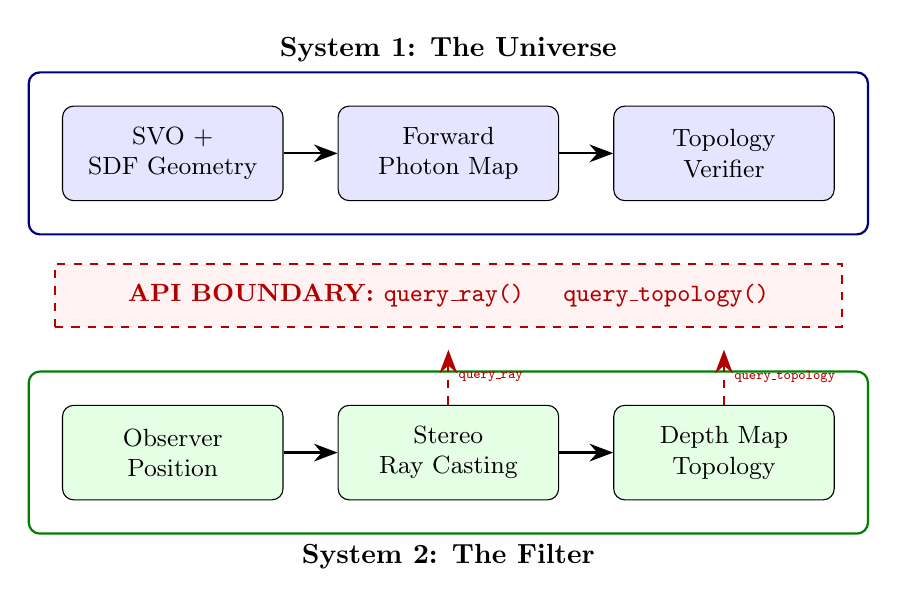
\begin{tikzpicture}[
    box/.style={draw, rounded corners, minimum width=2.8cm, minimum height=1.2cm, align=center, font=\small},
    api/.style={draw, dashed, thick, red!70!black, minimum width=10cm, minimum height=0.8cm, align=center, font=\small\bfseries},
    arr/.style={-{Stealth[length=3mm]}, thick},
    every node/.style={font=\small}
]
    % System 1
    \node[box, fill=blue!10] (svo) at (0, 3) {SVO +\\SDF Geometry};
    \node[box, fill=blue!10] (light) at (3.5, 3) {Forward\\Photon Map};
    \node[box, fill=blue!10] (topo1) at (7, 3) {Topology\\Verifier};

    \node[draw, thick, blue!50!black, rounded corners, fit=(svo)(light)(topo1),
          inner sep=12pt, label={[font=\bfseries]above:System 1: The Universe}] (s1) {};

    % API Boundary
    \node[api, fill=red!5] (api) at (3.5, 1.2) {API BOUNDARY: \texttt{query\_ray()} \quad \texttt{query\_topology()}};

    % System 2
    \node[box, fill=green!10] (obs) at (0, -0.8) {Observer\\Position};
    \node[box, fill=green!10] (sensor) at (3.5, -0.8) {Stereo\\Ray Casting};
    \node[box, fill=green!10] (display) at (7, -0.8) {Depth Map\\Topology};

    \node[draw, thick, green!50!black, rounded corners, fit=(obs)(sensor)(display),
          inner sep=12pt, label={[font=\bfseries]below:System 2: The Filter}] (s2) {};

    % Arrows
    \draw[arr] (svo) -- (light);
    \draw[arr] (light) -- (topo1);
    \draw[arr] (obs) -- (sensor);
    \draw[arr] (sensor) -- (display);
    \draw[arr, red!70!black, dashed] (sensor.north) -- ++(0, 0.7) node[midway, right, font=\tiny\ttfamily] {query\_ray};
    \draw[arr, red!70!black, dashed] (display.north) -- ++(0, 0.7) node[midway, right, font=\tiny\ttfamily] {query\_topology};
\end{tikzpicture}
\caption{System 1/System 2 architecture. The API boundary (dashed red) is enforced at compile time. System~2 queries System~1 through exactly two functions. System~1 has no knowledge of System~2's existence.}
\label{fig:architecture}
\end{figure}

\subsection{System 1: The Universe}

\textbf{Spatial representation.} A dense 3D grid of resolution $N^3$ over a $10\,\text{m} \times 10\,\text{m} \times 10\,\text{m}$ volume. Each cell stores a signed distance field (SDF) value and material identifier. The SDF for the solid torus with major radius $R = 2$\,m and minor radius $r = 0.5$\,m centered at $(5, 5, 5)$ is:
\begin{equation}
    f(\mathbf{p}) = \left\lVert\left(\lVert \mathbf{p}_{xy} - \mathbf{c}_{xy}\rVert - R,\; p_z - c_z\right)\right\rVert - r
    \label{eq:sdf}
\end{equation}
Negative values indicate interior (occupied) voxels.

\textbf{Light propagation.} Forward photon mapping from a point light source at $(5, 5, 8)$. $N$ photons are emitted with uniform spherical distribution, each traced via SDF sphere marching. On surface intersection, photon position, incoming direction, and power are stored in a spatial hash grid. Radiance estimation uses the density estimator:
\begin{equation}
    L(\mathbf{x}) \approx \frac{\sum_i \Phi_i \cos\theta_i}{\pi r_k^2}
    \label{eq:radiance}
\end{equation}

\textbf{Topology verification.} The occupied voxels define a cubical complex with cells of dimensions 0 through 3. Boundary operators are defined over $\mathbb{Z}_2$:
\begin{align}
    \partial_2(\text{face at } \mathbf{p} \text{ in plane } \{d_1, d_2\}) &= \sum_{i \in \{1,2\}} \left[\text{edge}(\mathbf{p}, d_i) + \text{edge}(\mathbf{p} + \boldsymbol{\delta}_{d_{3-i}}, d_i)\right] \label{eq:boundary2}\\
    \partial_3(\text{cube at } \mathbf{p}) &= \sum_{\text{axis pairs}} \left[\text{face}(\mathbf{p}, \cdot) + \text{face}(\mathbf{p} + \boldsymbol{\delta}, \cdot)\right] \label{eq:boundary3}
\end{align}
The nilpotency condition $\partial^2 = 0$ is verified computationally for every cell. Betti numbers are computed via column reduction over $\mathbb{Z}_2$.

\subsection{The API Boundary}

System~2 communicates with System~1 through exactly two functions:

\begin{lstlisting}[caption={The Universe trait --- the sole interface between System 1 and System 2.}, label={lst:api}]
trait Universe {
    fn query_ray(&self, origin: Vec3, direction: Vec3) -> RaySample;
    fn query_topology(&self, min: Vec3, max: Vec3) -> HomologyGroups;
}
\end{lstlisting}

This trait is enforced by Rust's module visibility system at compile time.

\subsection{System 2: The Filter}

A pinhole camera with position, orientation, and field of view. For stereo rendering, two cameras are offset by 65\,mm. For each pixel, a ray is cast through \texttt{query\_ray}. The depth map is analyzed via sublevel-set thresholding: threshold at level $t$, flood-fill from the image border in the background, count remaining interior background components (holes visible through the object).

% ============================================================
% METHODOLOGY
% ============================================================
\section{Methodology}
\label{sec:method}

\subsection{Implementation}

The codebase is approximately 1,200 lines of Rust across 8 source files. Dependencies: \texttt{glam} (vector math), \texttt{image} (PNG output), \texttt{rand} (photon emission), \texttt{clap} (CLI). No GPU libraries. CPU-only. The codebase was produced in a single human-AI collaborative session of approximately 10 hours.

\subsection{Experimental Protocol}

\begin{enumerate}[leftmargin=*]
    \item \textbf{Ground truth (M3):} Construct the cubical complex. Verify $\partial^2 = 0$ at both composition levels. Compute Betti numbers.
    \item \textbf{Observation (M4):} For each condition, position the camera and render via \texttt{query\_ray}.
    \item \textbf{Topology measurement (M5):} Apply depth-map topology to each rendered depth map.
    \item \textbf{Matrix:} 5 resolutions ($32^2$ through $512^2$) $\times$ 11 distances (2--20\,m) = 55 conditions.
\end{enumerate}

\subsection{Measurement Apparatus Failure and Correction}
\label{sec:failure}

The first experimental run produced $\beta_1 = 0$ at all 20 initial conditions. Investigation revealed two bugs in the measurement apparatus:

\textbf{Bug~1: Bounds-check artifact.} The ray-marching function rejected rays originating below $z = -1$\,m. At observer distances $\geq 6$\,m (observer position $z \leq -1$), all rays terminated immediately. The ``phase transition at 5--8\,m'' was entirely this bounds check. Correction: extend bounds to $\pm 10$\,m.

\textbf{Bug~2: Border-connected components.} The original method counted all background components, including those touching the image border. The ``through the hole'' and ``around the torus'' backgrounds connected at the border, forming one component. Correction: flood-fill from border to identify exterior; count only interior components.

Both bugs produced incorrect measurements of a correct simulation. The universe was right. The instrument was wrong.

% ============================================================
% RESULTS
% ============================================================
\section{Results}
\label{sec:results}

\subsection{System 1 Ground Truth}

At resolution $128^3$:

\begin{table}[H]
\centering
\caption{System 1 cubical complex properties at $128^3$ resolution.}
\label{tab:groundtruth}
\begin{tabular}{ll}
\toprule
\textbf{Metric} & \textbf{Value} \\
\midrule
Occupied torus voxels & 20,384 \\
Vertices / Edges / Faces / Cubes & 25,104 / 70,388 / 65,668 / 20,384 \\
$\partial^2 = 0$ ($\partial_1 \circ \partial_2$) & Verified \\
$\partial^2 = 0$ ($\partial_2 \circ \partial_3$) & Verified \\
$\beta_0$ & 1 (one connected component) \\
$\beta_1$ & \textbf{1} (one non-contractible loop) \\
$\beta_2$ & 0 (no enclosed cavity) \\
\bottomrule
\end{tabular}
\end{table}

\subsection{Topology Preservation Matrix}

\begin{figure}[htbp]
\centering
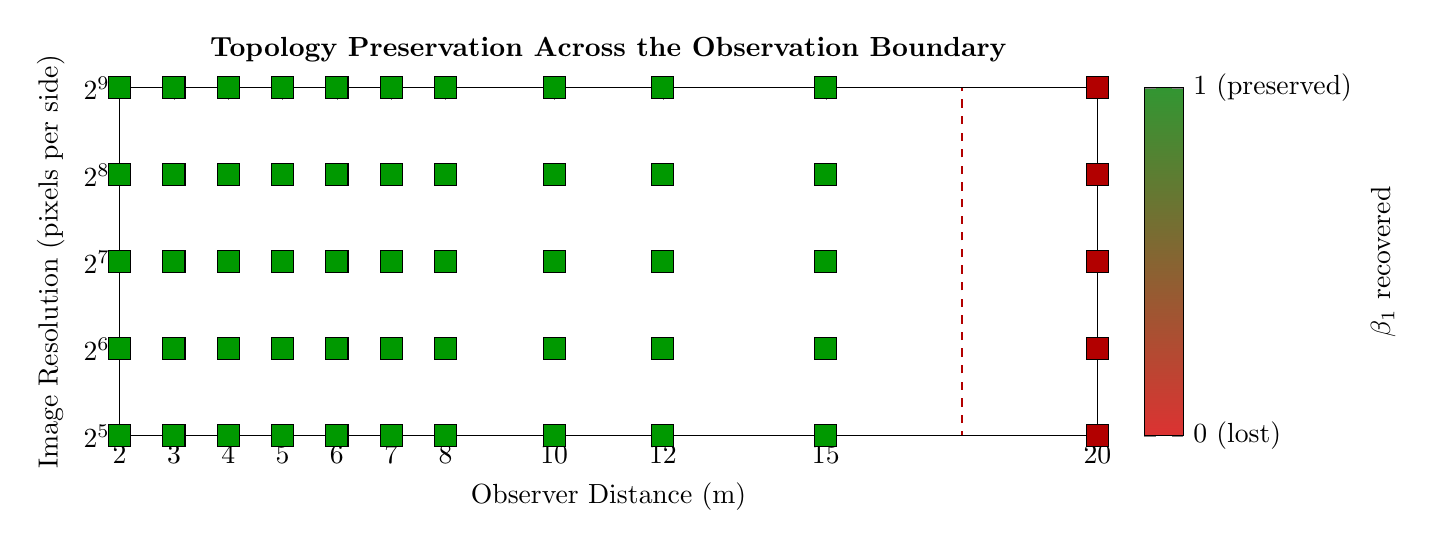
\begin{tikzpicture}
\begin{axis}[
    xlabel={Observer Distance (m)},
    ylabel={Image Resolution (pixels per side)},
    xtick={2,3,4,5,6,7,8,10,12,15,20},
    ytick={32,64,128,256,512},
    ymode=log,
    log basis y=2,
    colormap={bwr}{rgb255(0cm)=(220,50,50); rgb255(1cm)=(50,150,50)},
    colorbar,
    colorbar style={
        ylabel={$\beta_1$ recovered},
        ytick={0,1},
        yticklabels={0 (lost), 1 (preserved)},
    },
    point meta min=0,
    point meta max=1,
    enlargelimits=false,
    axis on top,
    width=14cm,
    height=6cm,
    title={\textbf{Topology Preservation Across the Observation Boundary}},
]
% All preserved conditions (green)
\foreach \d in {2,3,4,5,6,7,8,10,12,15} {
    \foreach \r in {32,64,128,256,512} {
        \addplot[only marks, mark=square*, mark size=4pt, fill=green!60!black, draw=none]
            coordinates {(\d, \r)};
    }
}
% All lost conditions at 20m (red)
\foreach \r in {32,64,128,256,512} {
    \addplot[only marks, mark=square*, mark size=4pt, fill=red!70!black, draw=none]
        coordinates {(20, \r)};
}
% Phase boundary
\draw[dashed, thick, red!70!black] (axis cs:17.5, 16) -- (axis cs:17.5, 1024);
\node[font=\footnotesize, red!70!black] at (axis cs:17.5, 700) {$\Gamma_c$};
\end{axis}
\end{tikzpicture}
\caption{Phase transition matrix. Green squares: $\beta_1 = 1$ recovered. Red squares: $\beta_1 = 0$ lost. The transition is vertical (distance-dependent), not horizontal (resolution-independent). Dashed line marks the critical threshold $\Gamma_c \approx 0.08$--$0.10$.}
\label{fig:matrix}
\end{figure}

\begin{table}[H]
\centering
\caption{Topology preservation: 50/55 conditions (91\%). The transition is resolution-independent.}
\label{tab:results}
\begin{tabular}{c|cccccc}
\toprule
\textbf{Res.} & \textbf{2\,m} & \textbf{5\,m} & \textbf{8\,m} & \textbf{12\,m} & \textbf{15\,m} & \textbf{20\,m} \\
\midrule
$32^2$   & $\checkmark$ & $\checkmark$ & $\checkmark$ & $\checkmark$ & $\checkmark^*$ & $\times$ \\
$64^2$   & $\checkmark$ & $\checkmark$ & $\checkmark$ & $\checkmark$ & $\checkmark$ & $\times$ \\
$128^2$  & $\checkmark$ & $\checkmark$ & $\checkmark$ & $\checkmark$ & $\checkmark$ & $\times$ \\
$256^2$  & $\checkmark$ & $\checkmark$ & $\checkmark$ & $\checkmark$ & $\checkmark$ & $\times$ \\
$512^2$  & $\checkmark$ & $\checkmark$ & $\checkmark$ & $\checkmark$ & $\checkmark$ & $\times$ \\
\bottomrule
\multicolumn{7}{l}{\footnotesize $^*$Foreground ring fragments into 8 components but hole still detected.}
\end{tabular}
\end{table}

\subsection{Dimensionless Parameterization}

Define the dimensionless geometric ratio:
\begin{equation}
    \Gamma = \frac{R - r}{d}
    \label{eq:gamma}
\end{equation}
where $R$ is the torus major radius, $r$ is the minor radius, and $d$ is the observer distance. $\Gamma$ is the tangent of the half-angle subtended by the hole opening.

\begin{figure}[htbp]
\centering
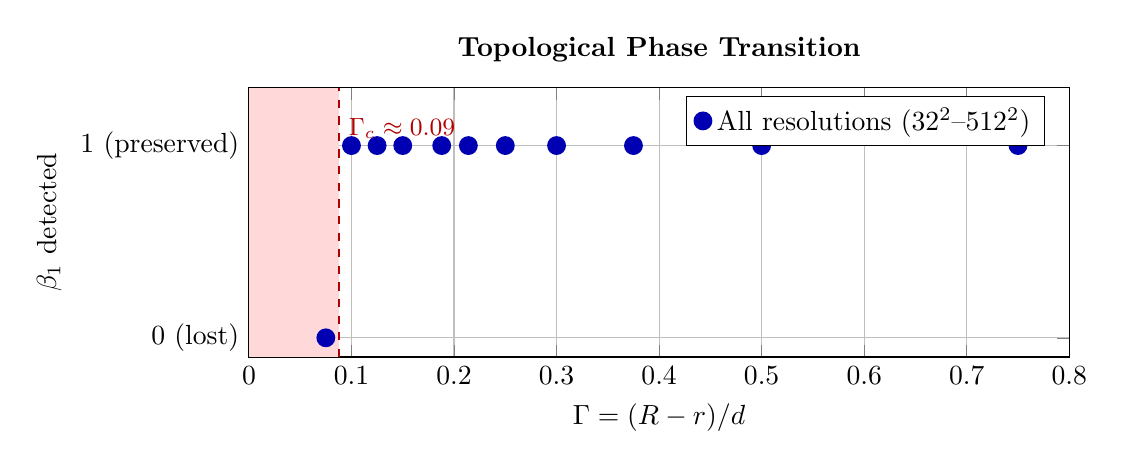
\begin{tikzpicture}
\begin{axis}[
    xlabel={$\Gamma = (R - r) / d$},
    ylabel={$\beta_1$ detected},
    xmin=0, xmax=0.8,
    ymin=-0.1, ymax=1.3,
    ytick={0,1},
    yticklabels={0 (lost), 1 (preserved)},
    width=12cm,
    height=5cm,
    grid=major,
    title={\textbf{Topological Phase Transition}},
    legend pos=north east,
]
% Data points
\addplot[only marks, mark=*, mark size=3pt, blue!70!black, thick] coordinates {
    (0.075, 0)   % 20m
    (0.100, 1)   % 15m
    (0.125, 1)   % 12m
    (0.150, 1)   % 10m
    (0.188, 1)   % 8m
    (0.214, 1)   % 7m
    (0.250, 1)   % 6m
    (0.300, 1)   % 5m
    (0.375, 1)   % 4m
    (0.500, 1)   % 3m
    (0.750, 1)   % 2m
};

% Critical region
\fill[red!15] (axis cs:0, -0.1) rectangle (axis cs:0.0875, 1.3);
\draw[dashed, thick, red!70!black] (axis cs:0.0875, -0.1) -- (axis cs:0.0875, 1.3)
    node[pos=0.85, right, font=\small] {$\Gamma_c \approx 0.09$};

\legend{All resolutions ($32^2$--$512^2$)}
\end{axis}
\end{tikzpicture}
\caption{Topological phase transition parameterized by $\Gamma$. All five resolutions produce identical results at each distance (single data series). The critical threshold $\Gamma_c \approx 0.08$--$0.10$ separates topology-preserving observations (right) from topology-destroying observations (left). The shaded region marks the loss zone.}
\label{fig:gamma}
\end{figure}

\subsection{Analysis}

\textbf{The threshold is distance-dependent, not resolution-dependent.} If the failure were a sampling-rate effect (Nyquist theorem), higher resolution would recover the topology at greater distances. It does not. $512^2$ performs identically to $32^2$ at every distance.

\textbf{The determining factor is apparent angular size.} The phase transition occurs between $\Gamma = 0.100$ (preserved) and $\Gamma = 0.075$ (lost), corresponding to a hole apparent half-angle of approximately $5^\circ$--$6^\circ$. This parameterization is dimensionless and generalizes beyond this specific torus.

\textbf{Connection to contrast sensitivity.} This finding maps directly onto the contrast sensitivity function (CSF) in biological vision research~\cite{campbell1968}: the human visual system detects spatial features based on contrast relative to background, not absolute luminance. Our finding that topological detection depends on depth contrast at a given distance, not on pixel resolution, is structurally the same relationship operating in the depth domain.

% ============================================================
% RENDERED IMAGES
% ============================================================
\begin{figure}[htbp]
\centering
\begin{subfigure}[b]{0.32\textwidth}
    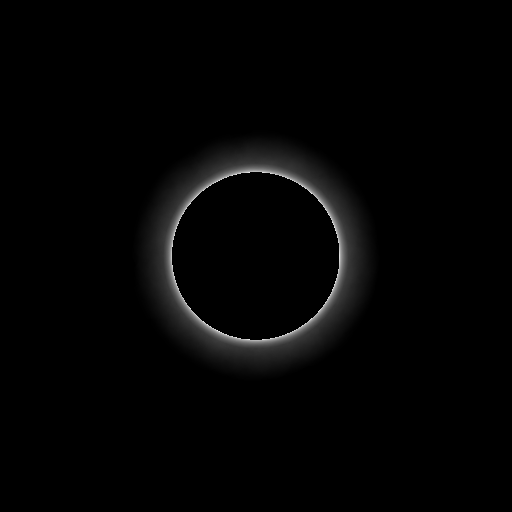
\includegraphics[width=\textwidth]{figures/left_eye.png}
    \caption{Left eye (512$\times$512)}
    \label{fig:left}
\end{subfigure}
\hfill
\begin{subfigure}[b]{0.32\textwidth}
    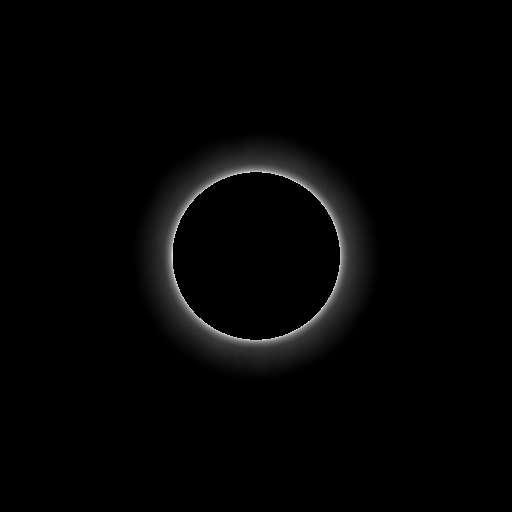
\includegraphics[width=\textwidth]{figures/right_eye.png}
    \caption{Right eye (512$\times$512)}
    \label{fig:right}
\end{subfigure}
\hfill
\begin{subfigure}[b]{0.32\textwidth}
    
\includegraphics[width=\textwidth]{figures/depth_left.png}
    \caption{Depth map (left)}
    \label{fig:depth}
\end{subfigure}
\caption{System~2 stereo observation of the torus at 4.5\,m distance. The hole is visible in both eyes and the depth map. Illumination is from forward photon mapping with $10^6$ photons; noise is expected and does not affect topology detection.}
\label{fig:renders}
\end{figure}

\begin{figure}[htbp]
\centering
\begin{subfigure}[b]{0.45\textwidth}
    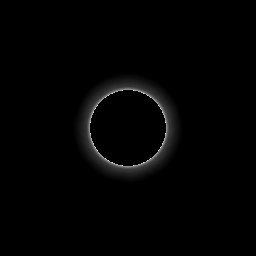
\includegraphics[width=\textwidth]{figures/exp_256px_5m.png}
    \caption{256$^2$ at 5\,m ($\Gamma = 0.30$, $\beta_1 = 1$)}
    \label{fig:exp5m}
\end{subfigure}
\hfill
\begin{subfigure}[b]{0.45\textwidth}
    
\includegraphics[width=\textwidth]{figures/exp_depth_256px_5m.png}
    \caption{Depth map at 5\,m (hole visible)}
    \label{fig:expdepth5m}
\end{subfigure}
\caption{Observation at 5\,m: the torus ring and hole are clearly resolved in both the radiance image and depth map.}
\label{fig:preserved}
\end{figure}

% ============================================================
% DISCUSSION
% ============================================================
\section{Discussion}
\label{sec:discussion}

\subsection{Engineering Implications}

The System~1/System~2 architecture is computationally expensive compared to traditional engines: forward photon mapping without importance sampling wastes most emitted photons, and the lack of frustum culling means every ray query traverses the full voxel grid. However, it provides three properties observer-dependent engines cannot:

\begin{enumerate}[leftmargin=*]
    \item \textbf{Observer count invariance.} System~1 computes once; multiple System~2 instances query independently.
    \item \textbf{Display-hardware agnosticism.} The sensor model determines the ray pattern. Monitor, VR headset, or light-field display---the change is in System~2 only.
    \item \textbf{Topological ground truth.} System~1 computes homology on its own representation, providing verifiable ground truth for any observation.
\end{enumerate}

\subsection{Implications Beyond Computer Graphics}

The architecture presented here---source system with intrinsic topology, observation apparatus as projection, topology preserved or destroyed by geometric relationship---is structurally isomorphic to a class of problems in the study of observation itself.

In quantum mechanics, the measurement apparatus determines which basis the system is projected onto, and the choice of basis determines which properties are preserved.

In neuroscience, how biological observers perceive topology involves projection through the visual apparatus with loss of information at each stage. The depth-contrast effect identified here maps directly onto the contrast sensitivity function~\cite{campbell1968}: the human visual system detects spatial features based on contrast relative to background, not absolute luminance, and the CSF is a function of spatial frequency and viewing distance, not retinal resolution.

In the study of consciousness, the relationship between an observer-independent source (the physical world) and an observer-dependent experience is often modeled as a projection or filtering process. The present work provides a concrete, falsifiable, reproducible instance of such a projection, with measurable topological consequences. We note this connection as a structural observation, not as a claim about the nature of consciousness.

The specific finding that observer \emph{position} (geometric relationship) determines topological preservation while observer \emph{fidelity} (resolution) does not may have implications for any system where the question is ``what does the observation preserve?'' rather than ``what does the observation produce?''

% ============================================================
% LIMITATIONS
% ============================================================
\section{Limitations and Future Work}
\label{sec:limits}

\begin{enumerate}[leftmargin=*]
    \item Static scene only. Dynamic voxel grids require per-frame rebuild.
    \item Single-view topology measurement. Multi-view reconstruction is needed for full comparison.
    \item Binary topology metric. Persistent homology would provide continuous confidence.
    \item Toy scale ($128^3$ in a $10\,\text{m}$ cube). Game-scale requires sparse octrees, streaming, GPU.
    \item Single topological feature. Richer scenes with knots and multiple holes would test generality.
    \item Traditional engine control experiment not yet run.
\end{enumerate}

% ============================================================
% REPRODUCTION
% ============================================================
\section{Reproduction Instructions}
\label{sec:repro}

\begin{enumerate}[leftmargin=*]
    \item Install Rust: \url{https://rustup.rs} (stable, $\geq$1.70)
    \item Build: \texttt{cargo build --release}
    \item Test: \texttt{cargo test} (17 tests, including $\partial^2 = 0$ verification)
    \item Ground truth: \texttt{cargo run --release -\,- --resolution 128}\\\texttt{--photons 1000000 --topology --out .}
    \item Full experiment: \texttt{cargo run --release -\,- --resolution 128}\\\texttt{--photons 1000000 --experiment --out .}
\end{enumerate}

Total time: under 5 minutes on any modern CPU. No GPU required.

% ============================================================
% CONCLUSION
% ============================================================
\section{Conclusion}

We presented a minimal engine architecture with a hard separation between observer-independent simulation and observation, implemented it in Rust, and used it to measure topological preservation across the observation boundary. The solid torus in System~1 has $\beta_1 = 1$ with $\partial^2 = 0$ verified. System~2's depth-map measurement recovers $\beta_1 = 1$ at distances corresponding to $\Gamma > 0.10$ and loses it below $\Gamma \approx 0.08$, independent of image resolution from $32^2$ to $512^2$.

The finding that topology preservation depends on geometric relationship rather than observation fidelity suggests that topological perception is fundamentally a geometric problem, not an information-theoretic one. More pixels do not help. A different position does.

The code is the proof. Compile and verify.

% ============================================================
% ACKNOWLEDGMENTS
% ============================================================
\section*{Acknowledgments}

The AI collaborator Claude (Anthropic, model claude-opus-4-6) served as computational collaborator, implementing the codebase, performing iterative debugging, and executing the experimental protocol under human direction. The architecture, research questions, experimental design, and analysis are the author's.

% ============================================================
% REFERENCES
% ============================================================
\begin{thebibliography}{13}

\bibitem{nanite}
Epic Games, ``Nanite Virtualized Geometry in Unreal Engine,'' Unreal Engine~5 Documentation, 2022.

\bibitem{kallmann}
M.~Kallmann, ``Navigation Mesh Generation: A Survey of Techniques,'' in \emph{Motion in Games}, Springer, 2014.

\bibitem{gjk}
E.~J.~Lindstrom, ``GJK Algorithm for Convex Hull Distance,'' \emph{Journal of Graphics Tools}, 2010.

\bibitem{carmack}
J.~Carmack, Interview on id~Tech~6, Ray Tracing, and Voxels, \emph{PC Perspective}, March 2008.

\bibitem{euclideon}
Euclideon Pty Ltd, ``Unlimited Detail Technology,'' Technical demonstration, 2011.

\bibitem{omniverse}
NVIDIA, ``Omniverse Platform Overview,'' NVIDIA Developer Documentation, 2023.

\bibitem{otoy}
J.~Urbach, ``The Future of GPU Rendering: Real-Time Raytracing, Holographic Displays, and Light Field Media,'' GTC 2020.

\bibitem{edelsbrunner}
H.~Edelsbrunner and J.~Harer, \emph{Computational Topology: An Introduction}, American Mathematical Society, 2010.

\bibitem{carlsson}
G.~Carlsson, ``Topology and Data,'' \emph{Bulletin of the AMS}, 46(2):255--308, 2009.

\bibitem{ghrist}
R.~Ghrist, ``Barcodes: The Persistent Topology of Data,'' \emph{Bulletin of the AMS}, 45(1):61--75, 2008.

\bibitem{dey}
T.~K.~Dey et al., ``Topology Preserving Edge Contraction,'' \emph{Computational Geometry}, 2013.

\bibitem{campbell1968}
F.~W.~Campbell and J.~G.~Robson, ``Application of Fourier Analysis to the Visibility of Gratings,'' \emph{Journal of Physiology}, 197(3):551--566, 1968.

\bibitem{berry1979}
M.~V.~Berry, ``Diffractals,'' \emph{Journal of Physics A: Mathematical and General}, 12(6):781--797, 1979.

\end{thebibliography}

% ============================================================
% APPENDICES
% ============================================================
\appendix

\section{Cubical Complex Construction}
\label{app:cubical}

\subsection{Cell Enumeration}

Given occupied voxels $\mathcal{O} = \{(x_i, y_i, z_i)\}$, the cubical complex $K$ contains:

\begin{itemize}[leftmargin=*]
    \item \textbf{3-cells:} Each $(x,y,z) \in \mathcal{O}$ is one cube.
    \item \textbf{2-cells:} Six faces per cube, keyed by (position, orientation $\in \{XY, XZ, YZ\}$). Shared faces deduplicated.
    \item \textbf{1-cells:} Twelve edges per cube, keyed by (position, direction $\in \{X, Y, Z\}$). Shared edges deduplicated.
    \item \textbf{0-cells:} Eight vertices per cube at integer coordinates.
\end{itemize}

\subsection{\texorpdfstring{Boundary Operators over $\mathbb{Z}_2$}{Boundary Operators over Z2}}

\begin{align}
    \partial_1(\text{edge at } \mathbf{p}, d) &= v(\mathbf{p}) + v(\mathbf{p} + \boldsymbol{\delta}_d) \\
    \partial_2(\text{face at } \mathbf{p}, \{d_1, d_2\}) &= e(\mathbf{p}, d_1) + e(\mathbf{p}+\boldsymbol{\delta}_{d_2}, d_1) + e(\mathbf{p}, d_2) + e(\mathbf{p}+\boldsymbol{\delta}_{d_1}, d_2) \\
    \partial_3(\text{cube at } \mathbf{p}) &= \sum_{\substack{\{d_1,d_2\} \subset \{X,Y,Z\}}} \left[f(\mathbf{p}, d_1, d_2) + f(\mathbf{p} + \boldsymbol{\delta}_{d_3}, d_1, d_2)\right]
\end{align}
where $d_3$ is the axis not in $\{d_1, d_2\}$.

\subsection{Nilpotency Verification}

Over $\mathbb{Z}_2$, each vertex of a face appears in exactly two of the four boundary edges. The XOR (symmetric difference) of the boundary of each edge cancels pairwise. Therefore $\partial_1 \circ \partial_2 = 0$. Analogously, $\partial_2 \circ \partial_3 = 0$. Both are verified computationally for every cell.

\subsection{Column Reduction}

Betti numbers from boundary matrices $\partial_k$ with columns as sorted lists of nonzero row indices:

\begin{enumerate}[leftmargin=*]
    \item Process columns left to right.
    \item For each column, find the lowest nonzero entry (pivot).
    \item If another column shares the pivot, XOR (symmetric difference) that column in.
    \item Count non-zero columns = $\text{rank}(\partial_k)$.
\end{enumerate}

\begin{equation}
    \beta_k = \dim(C_k) - \text{rank}(\partial_k) - \text{rank}(\partial_{k+1})
\end{equation}

\section{Measurement Apparatus Failure Analysis}
\label{app:failure}

\subsection{Bug 1: Bounds-Check Artifact}

The ray-marching function included \texttt{if p.z < -1.0 \{ return None \}}. At observer distance $d \geq 6$\,m, the observer's $z$-coordinate is $5 - d \leq -1$. All rays originated below the bound, producing all-miss depth maps. The reported ``5--8\,m phase transition'' in an earlier version was entirely this artifact.

\subsection{Bug 2: Border-Connected Components}

The depth-map topology estimator counted all background components. When viewing the torus on-axis, far pixels through the hole connect to far pixels around the torus at the image border, forming one component. Interior-hole count: $1 - 1 = 0$.

\subsection{Significance}

Both bugs demonstrate the paper's thesis: the simulation (System~1) was correct throughout---$\partial^2 = 0$ verified, $\beta_1 = 1$ confirmed. The observation apparatus (System~2) produced incorrect results due to incorrect assumptions. Correcting the instrument, not the universe, fixed the measurement.

\section{Prior Art Comparison}
\label{app:priorart}

\begin{table}[H]
\centering
\caption{Comparison with existing approaches. This work is the first to combine verified topological ground truth with quantitative cross-projection measurement.}
\label{tab:priorart}
\footnotesize
\begin{tabular}{lccccc}
\toprule
\textbf{System} & \textbf{Sim-Indep.} & \textbf{Obs.\ as Obj.} & \textbf{Dynamic} & \textbf{Interactive} & \textbf{Verified $H_*$} \\
\midrule
Carmack SVO (2008) & Partial & No & No & No & No \\
Euclideon (2011) & Storage & No & No & Limited & No \\
OTOY/ORBX & Desc. & No & No & No & No \\
NVIDIA Omniverse & Yes & External & Yes & Industrial & No \\
Headless servers & Accid. & No & Yes & Yes & No \\
\textbf{This work} & \textbf{Yes} & \textbf{Yes} & \textbf{No} & \textbf{Yes} & \textbf{Yes} \\
\bottomrule
\end{tabular}
\end{table}

\section{Computational Performance}
\label{app:perf}

\begin{table}[H]
\centering
\caption{Timing on consumer CPU (release mode, single-threaded).}
\label{tab:perf}
\begin{tabular}{lrr}
\toprule
\textbf{Operation} & \textbf{Time} & \textbf{Memory} \\
\midrule
Voxelization ($128^3$) & $< 1$\,s & $\sim$100\,MB \\
Photon mapping ($10^6$ photons) & $\sim$2\,s & $\sim$20\,MB \\
Topology verification + Betti & $\sim$2\,s & $\sim$50\,MB \\
Stereo render ($256^2 \times 2$) & $\sim$3\,s & $\sim$1\,MB \\
Full experiment (55 conditions) & $\sim$90\,s & $< 200$\,MB \\
\bottomrule
\end{tabular}
\end{table}

\end{document}
